% !TeX root = ../main.tex
\chapter{背景知識與文獻探討}\label{chapter:background}

    此章將介紹本研究相關的文獻與背景知識,包含超音波麥克風干擾器、噪音消除技術與存取控制。


\section{超音波麥克風干擾器}\label{section:background-jammer}

    超音波麥克風干擾器的發明旨在解決竊聽的問題,例如:在未經允許的前提下,以隱密的方式紀錄不對外公開的私人對話。
錄音是一種常見的竊聽方式,在智慧型設備普及的現代,由於有能力錄音設備體積很小,例如:錄音筆、智慧手機與智慧手錶等。
攻擊者可以輕鬆地在機密會議和私人談話中,在未經會談參與者允許前提下,透過錄音記錄秘密聲音訊息。
因此,保護機密會議和私人談話,避免遭非允許錄製對於個人語音談話、商業貿易甚至國家安全都非常重要。

    為了解決上述問題,最近的工業產品與學術研究\cite{chen2020wearable}顯示,可以利用超音波產生噪音來干擾錄音。
麥克風的工作原理就像人的耳朵,如果播放可聽見的聲音(20Hz~20kHz),人類的耳朵與和麥克風都將能夠聽到它。
若果播放的聲音是超音波(20kHz以上),此頻率超過人類耳朵的聽力範圍因此聽不到,但可以被麥克風聽到。
基於此原理 Roy 等人提出了一種稱為 BackDoor 的超音波干擾技術,利用麥克風對於超音波的非線性響應輸出特性將噪音注入麥克風。
透過播放特別設計構造的超音波,可以對麥克風執行拒絕服務 (DoS) 攻擊\cite{roy2017backdoor}。
其中若對於麥克風的非線性響應輸出產生的噪音的幅度若大於人聲的幅度,
錄音設備就只能記錄噪音,人與人的對談聲幾乎無法識別\cite{shen2019jamsys}。
以此即可保持會談內容隱私必免遭到錄音竊聽,而解決非法取得有效之聲音記錄的問題。

    為優化超音波麥克風干擾器的效率,Yuxin Chen 等人提出,
透過將超音波麥克風干擾器製造成環形穿戴裝置,可以有效的解決干擾死角的問題\cite{chen2020demonstrating}。
並且解釋了超音波麥克風干擾器對於麥克風的非線性響應輸出其原理為麥克風系統為一複雜的組成的不可知系統,
會將高頻的聲音能量轉換投影至人耳可聽見頻率內,而產生噪音干擾\cite{chen2019understanding}。
另外,Hao Shen 等人也提出於多麥克風超音波干擾器的情境中,
透過改變擺放位置與角度的變化優化超音波麥克風干擾器的效率\cite{shen2019jamsys}。


\section{主動式噪音消除技術}\label{section:background-anc}

    主動式噪音消除(Active Noise Cancellation, ANC) 或又稱主動式噪音控制(Active Noise Control, ANC),
是一種用來消除噪音的方法。其原理為透過產生與噪音極性反轉的波(polarity inversion),利用兩波的抵銷干涉來消除噪音。
此概念最早於 1963 由 Paul Lueg 提出 \cite{elliott1993active}。
現代實際應用中,由於傳統濾波器中的參數是固定的,因此無法有效處理非穩態(Non-Stationarity)噪音。
透過自適應濾波器(Adaptive filter),可以增加濾波器自我調節的能力來解決上述問題。
自適應濾波器為一類線性濾波器,其組成為一遞移函數(Transfer function)包含多個可控參數,
根據參考訊號的變化透過優化演算法(optimization algorithm)來更新函數中的可控參數。
此設計得以使濾波器獲得自適應的能力,得以有效的處理未知的響應輸出系統\cite{widrow1983adaptive}。

    將自適應濾波器應用於主動式噪音消除,又稱為自適應噪音消除(Active Noise Cancellation, ANC),
為一種消除訊號中的破壞性干擾的一種方法。
透過被干擾訊號作為主要輸入和包含與主要輸入中的噪音高度相關的參考輸入。
將參考輸入透過自適應濾波器轉換後並從主要輸入中減去以獲得還原噪音消除的訊號。
最小均方濾波器(Least Mean Square Filter, LMS Filter) 為一類自適應濾波器,
其原理為將LMS演算法應用至自適應濾波器中的優化演算法,最小化產生訊號與目標訊號之間的差\cite{widrow1975adaptive}。

    自適應濾波器允許處理確定性或隨機性、平穩性或時間變量的輸入。
此解決方案表明,當參考輸入與欲消除的破壞性干擾噪音高度相關時,可以消除主要輸入中的噪音而不會產生訊號失真。
若處理週期性干擾時,自適應噪音消除器可以作為帶通濾波器(Band-pass filter),且具有跟踪干擾準確頻率的能力。
在這種情況下,消除器表現為線性、時不變系統,自適應濾波器收斂於動態結果而非靜態結果。
實驗結果說明了自適應噪音消除技術在各種實際應用中的有用性\cite{singh2001adaptive}。

\begin{figure}[H]
    \centering
    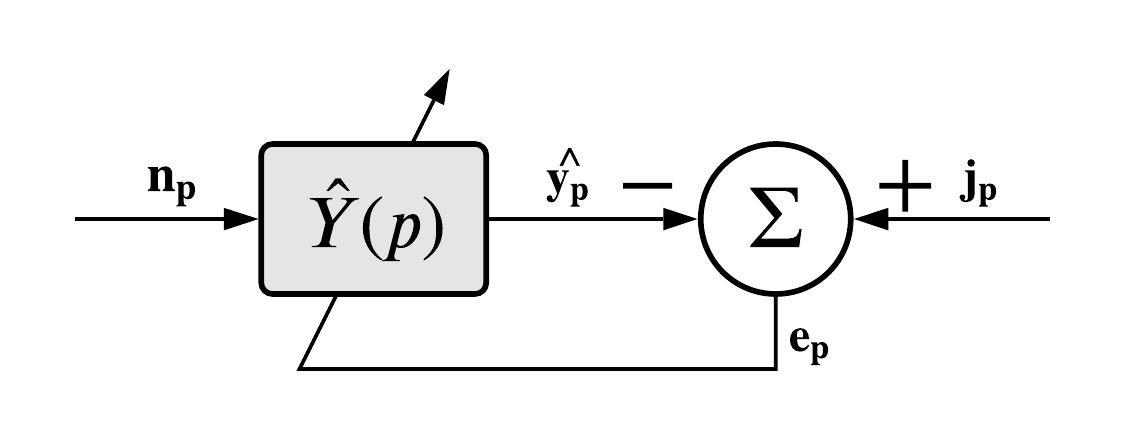
\includegraphics[width=0.45\textwidth]{af}
    \caption{自適應濾波器}\label{fig:af}
\end{figure}

    基本的 LMS 存在著許多缺點,例如其對於主要輸入的幅度過於敏感。
歸一化最小均方濾波器(Normalized least mean squares filter, NLMS)的提出旨在解決上述問題。
其原理為透過輸入訊號的功率歸一化,來降低對於主要輸入的波形震幅敏感度\cite{book198585}。
其他改良方向例如:可變步進值LMS(Variable Step-Size, VSS-LMS) \cite{kwong1992variable}。


\section{存取控制}\label{section:background-access-control}

    存取控制(Access Control)是對一個資源的存取的選擇性限制\cite{rfc4949},而存取控制描述了這個過程。
其的目的為保護系統資源免受未經授權的存取,存取的行為可能代表著消費、進入或使用。
存取資源的權限稱為授權\cite{sandhu1994access}。

    金鑰分割是一種向一組參與者之間分發秘密的方法,每個參與者都被分配了一份秘密,
只有當足夠數量的授權的子集才能重建秘密。
金鑰分割是密碼學中的重要工具,它們被用作許多安全協議的構建基礎,
例如安全多方計算(Secure Multi-Party Computation)、拜占庭協議(Byzantine agreement)、
閾值密碼系統(Threshold cryptosystem)、存取控制等\cite{beimel2011secret}。
在金鑰分割情境中有一個分發者和 $n$ 個參與者,分發者將秘密的一部分分享給參與者,
但只有在滿足特定條件時,參與者才能從他們的份額中重建秘密。
當滿足任何一組數量大於 $t$(閾值)時,參與者可以一起重建秘密,
如參與者數量小於閾值,則沒有機會重建秘密。
這樣的系統稱為 $(t , n )$ - 閾值方法(threshold scheme),
而 $n$ 個參與者則稱存取控制組(access control group)\cite{chum2012proposed}。

    若將金鑰分割應用於存取控制,可以用來保護使用委外資料(Outsourcing Data)。
在考慮經濟性、效率性和安全性的前提下,越來越多的中小型企業和自治組織正在嘗試將其不斷增長的業務資料,
使用委外資料的模式外包給一個或多個專業的存儲服務提供商。
但實際資料所有者和運營商的分離導致了對安全分佈式存儲技術的需求。
在這種情鏡中,無法如傳統存取控制模型中,假設執行存取控制策略的實體也是資料或資源的擁有者。
為解決上述問題,透過金鑰分割即可實現對於委外資料的存取控制
\cite{naor1998access}\cite{hadavi2016access}\cite{zhang2016privacy}。